\documentclass{fkssolpub}

\usepackage[czech]{babel}
\usepackage{fontspec}
\usepackage{fkssugar}
\usepackage{amsmath}
\usepackage{graphicx}

\newcommand{\dd}{\mathrm{d}}
\renewcommand{\angle}{\sphericalangle}

\author{Ondřej Sedláček}
\school{Gymnázium Oty Pavla} 
\series{4}
\problem{3} 

\begin{document}

\begin{figure}[h!]
  \begin{center}
    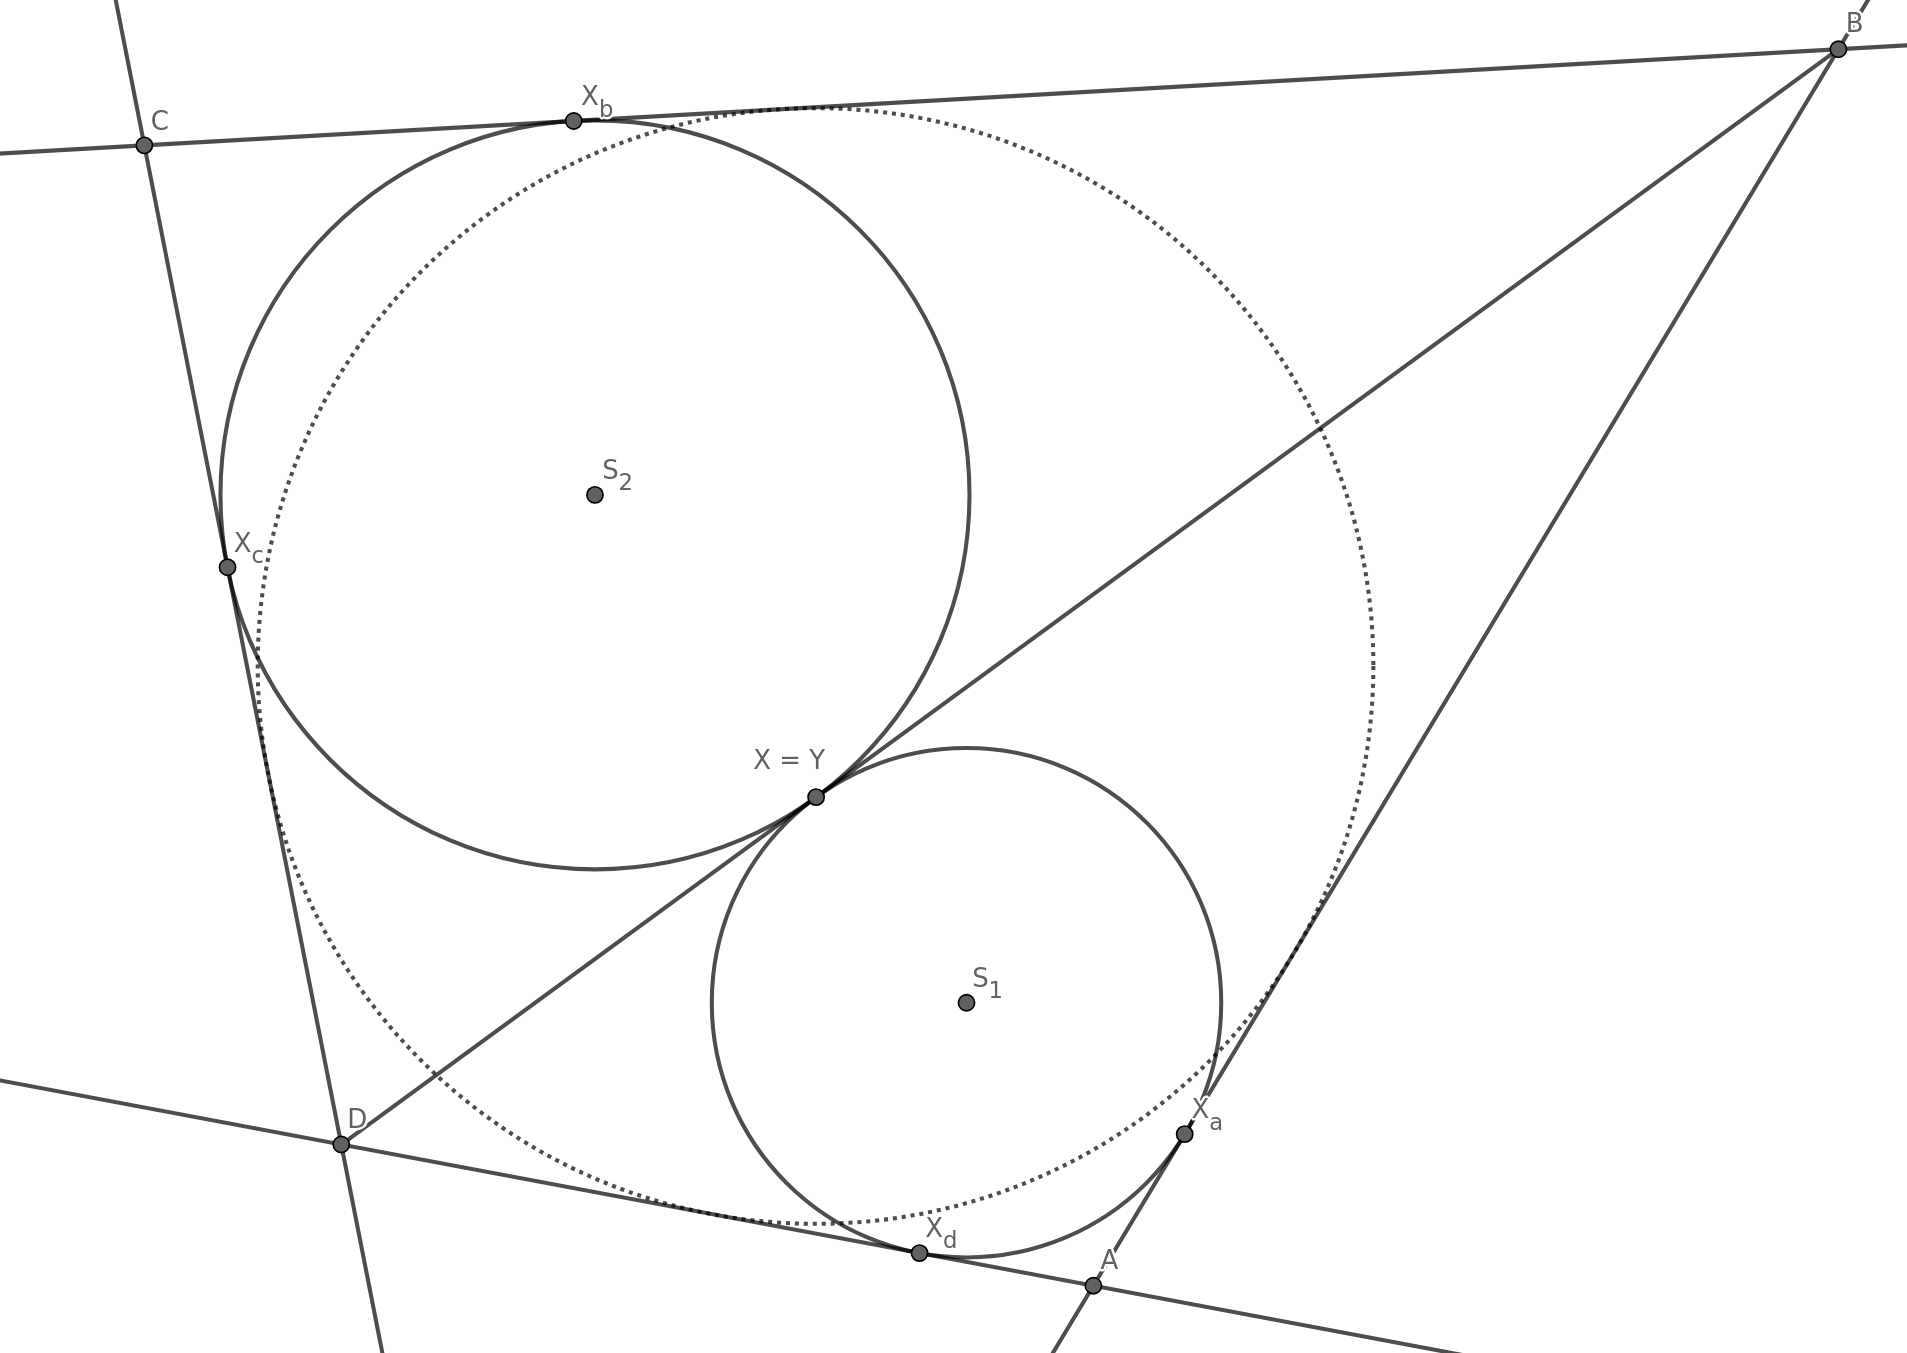
\includegraphics[width=0.95\textwidth]{3-fig.png}
  \end{center}
  \caption{K vysvětlení důkazu a značení}\label{fig:}
\end{figure}


Víme, že pro tečnové čtyřúhelníky platí rovnost:

\[
  |AB| + |CD| = |BC| + |AD|
\]

Z úsekových úhlů víme, že tečny vytvářejí rovnoramenné trojúhelníky, a to trojúhelníky z dotykových bodů tečen a jejich průsečíku. To můžeme využít k úpravě této rovnice:

\[
  |AX_a| + |X_aB| + |CX_c| + |X_cD| = |BX_b| + |X_bC| + |DX_d| + |X_dA|
\]
\[
  |AX_a| + |BX| + |CX_c| + |DY| = |BY| + |CX_c| + |DX| + |AX_a|
\]
\[
  |BX| + |DY| = |BY| + |DX|
\]
\[
  |BD| + |BX| - |BY| = |BD| + |BY| - |BX|
\]
\[
  |BX| = |BY|
\]

Tato rovnice zjevně platí jenom tehdy, pokud $X = Y$, protože oba body $X$ a $Y$ leží na úsečce $BD$. Tím jsme dokázali to, co jsme chtěli. Q. E. D.

\end{document}
